

%----------
% DOCUMENT CONFIGURATION
%----------

\documentclass[12pt]{report} %font 12pt

% MARGINS
\usepackage[
a4paper,
vmargin=2.5cm,
hmargin=3cm
]{geometry}

\renewcommand{\baselinestretch}{1.15}
\parskip=6pt

% COLORS for cover and code
\usepackage[table]{xcolor}
\definecolor{azulUC3M}{RGB}{0,0,102}
\definecolor{gray97}{gray}{.97}
\definecolor{gray75}{gray}{.75}
\definecolor{gray45}{gray}{.45}

% Soporte para GENERAR PDF/A --es importante de cara a su inclusión en e-Archivo porque es el formato óptimo de preservación y a la generación de metadatos, tal y como se describe en http://uc3m.libguides.com/ld.php?content_id=31389625. En la carpeta incluímos el archivo plantilla_tfg_2017.xmpdata en el que puedes incluir los metadatos que se incorporarán al archivo PDF cuando lo compiles. Ese archivo debe llamarse igual que tu archivo .tex. Puedes ver un ejemplo en esta misma carpeta.
\usepackage[a-1b]{pdfx}

% LINKS
\usepackage{hyperref}
\hypersetup{colorlinks=true,
	linkcolor=black,
	urlcolor=blue}

% MATH
\usepackage{amsmath,amssymb,amsfonts,amsthm}

\usepackage{txfonts} 
\usepackage[T1]{fontenc}
\usepackage[utf8]{inputenc}

\usepackage[english]{babel} 
\usepackage[babel, english=american]{csquotes}
\AtBeginEnvironment{quote}{\small}

% FOOTER
\usepackage{fancyhdr}
\pagestyle{fancy}
\fancyhf{}
\renewcommand{\headrulewidth}{0pt}
\rfoot{\thepage}
\fancypagestyle{plain}{\pagestyle{fancy}}

% TITLES
\usepackage{titlesec}
\usepackage{titletoc}
\titleformat{\chapter}[block]
{\large\bfseries\filcenter}
{\thechapter.}
{5pt}
{\MakeUppercase}
{}
\titlespacing{\chapter}{0pt}{0pt}{*3}
\titlecontents{chapter}
[0pt]                                               
{}
{\contentsmargin{0pt}\thecontentslabel.\enspace\uppercase}
{\contentsmargin{0pt}\uppercase}                        
{\titlerule*[.7pc]{.}\contentspage}                 

\titleformat{\section}
{\bfseries}
{\thesection.}
{5pt}
{}
\titlecontents{section}
[5pt]                                               
{}
{\contentsmargin{0pt}\thecontentslabel.\enspace}
{\contentsmargin{0pt}}
{\titlerule*[.7pc]{.}\contentspage}

\titleformat{\subsection}
{\normalsize\bfseries}
{\thesubsection.}
{5pt}
{}
\titlecontents{subsection}
[10pt]                                               
{}
{\contentsmargin{0pt}                          
	\thecontentslabel.\enspace}
{\contentsmargin{0pt}}                        
{\titlerule*[.7pc]{.}\contentspage}  


% TABLE DESIGN
\usepackage{multirow}
\usepackage{caption}
\usepackage{floatrow} 
\usepackage{array}
\newcolumntype{P}[1]{>{\centering\arraybackslash}p{#1}}
\DeclareCaptionFormat{upper}{#1#2\uppercase{#3}\par}

\captionsetup[table]{
	format=upper,
	justification=centering,
	labelsep=period,
	width=.75\linewidth,
	labelfont=small,
	font=small,
}



% FIGURES DESIGN
\usepackage{graphicx}
\graphicspath{{images/}}

\captionsetup[figure]{
	format=hang,
	name=Fig.,
	singlelinecheck=off,
	labelsep=period,
	labelfont=small,
	font=small,
	%THE FOLLOWING WAS ADDED BY ME, is this ok? I think it was missed on the template
	justification=centering		
}


% FOOT NOTES
\usepackage{chngcntr}
\counterwithout{footnote}{chapter}

% CODE LISTINGS
\usepackage{listings}

\lstdefinestyle{estilo}{ frame=Ltb,
	framerule=0pt,
	aboveskip=0.5cm,
	framextopmargin=3pt,
	framexbottommargin=3pt,
	framexleftmargin=0.4cm,
	framesep=0pt,
	rulesep=.4pt,
	backgroundcolor=\color{gray97},
	rulesepcolor=\color{black},
	%
	basicstyle=\ttfamily\footnotesize,
	keywordstyle=\bfseries,
	stringstyle=\ttfamily,
	showstringspaces = false,
	commentstyle=\color{gray45},     
	%
	numbers=left,
	numbersep=15pt,
	numberstyle=\tiny,
	numberfirstline = false,
	breaklines=true,
	xleftmargin=\parindent
}

\captionsetup[lstlisting]{font=small, labelsep=period}

\lstset{style=estilo}
\renewcommand{\lstlistingname}{\uppercase{Código}}

% IEEE BIBLIOGRAPHY
\usepackage[backend=biber, style=ieee, isbn=false,sortcites, maxbibnames=5, minbibnames=1]{biblatex}

\addbibresource{bibliography/bibliography.bib}


%-------------
%	DOCUMENT
%-------------

\begin{document}
\pagenumbering{roman}
	
%----------
%	COVER
%----------	
\begin{titlepage}
	\begin{sffamily}
	\color{azulUC3M}
	\begin{center}
		\begin{figure}[H] %university logotype
			\makebox[\textwidth][c]{
\includegraphics[width=16cm]{Portada_Logo.png}}
		\end{figure}
		\vspace{2.5cm}
		\begin{Large}
			University Degree in Computer Science and Engineering\\			
			Academic Year 2021-2022\\
			\vspace{2cm}		
			\textsl{Bachelor Thesis}
			\bigskip
			
		\end{Large}
		 	{\Huge ``An analysis of offensive capabilities of eBPF''}\\
		 	\vspace*{0.5cm}
	 		\rule{10.5cm}{0.1mm}\\
			\vspace*{0.9cm}
			{\LARGE Marcos Sánchez Bajo}\\ 
			\vspace*{1cm}
		\begin{Large}
			Juan Manuel Estévez Tapiador\\
			Leganés, 2022\\
		\end{Large}
	\end{center}
	\vfill
	\color{black}
	% Creative Commons license
	
\includegraphics[width=4.2cm]{images/creativecommons.png}\\  
	This work is licensed under Creative Commons \textbf{Attribution – Non Commercial – Non Derivatives}
	\end{sffamily}
\end{titlepage}

\newpage
\thispagestyle{empty}
\mbox{}

%----------
%	SUMMARY & KEYWORDS
%----------	
\renewcommand\abstractname{\large\uppercase{Summary}}
\begin{abstract}
\thispagestyle{plain}
\setcounter{page}{3}
	
	% TODO SUMMARY
	
	\textbf{Keywords:}
	% TODO KEYWORDS
	
	\vfill
\end{abstract}
	\newpage
	\thispagestyle{empty}
	\mbox{}


%----------
%	DEDICATION
%----------	
\chapter*{Dedication}

\setcounter{page}{5}
	
	% TODO DEDICATION	
		
	\vfill
	
	\newpage
	\thispagestyle{empty}
	\mbox{}
	
\chapter*{Abstract}

\setcounter{page}{5}
	
	% TODO ABSTRACT	
		
	\vfill
	
	\newpage
	\thispagestyle{empty}
	\mbox{}
	

%----------
%	INDEXES
%----------	

%--
%General indexes
%-
\tableofcontents
\thispagestyle{fancy}

\newpage
\thispagestyle{empty}
\mbox{}

%--
% List of figures
%-
\listoffigures
\thispagestyle{fancy}

\newpage
\thispagestyle{empty}
\mbox{}

%--
% List of tables
%-
\listoftables
\thispagestyle{fancy}

\newpage % página en blanco o de cortesía
\thispagestyle{empty}
\mbox{}


%----------
%	INTRODUCTION
%----------	
\clearpage
\pagenumbering{arabic}

\chapter{Introduction}
\section{Motivation}
%M-> SA bit long, but it summarizes and presents the ideas and background needed to understand the topic in order:
% Main idea: Malware keeps evolving -> 
% -> Relevance of innovating and researching on the new techniques ->
% -> Relevance of stealth software in targeted attacks-> 
% -> Introduce eBPF as the logical step of innovation in the field ->
% -> There is a need to research on this topic now.

As the efforts of the computer security community grow to protect increasingly critical devices and networks from malware infections, so do the techniques used by malicious actors become more sophisticated. Following the incorporation of ever more capable firewalls and Intrusion Detection Systems (IDS), cybercriminals have in turn sought novel attack vectors and exploits in common software, taking advantage of an inevitably larger attack surface that keeps growing due to the continued incorporation of new programs and functionalities into modern computer systems.

In contrast with ransomware incidents, which remained the most significant and common cyber threat faced by organizations on 2021\cite{ransomware_pwc}, a powerful class of malware called rootkits is found considerably more infrequently, yet it is usually associated to high-profile targeted attacks that lead to greatly impactful consequences. 

A rootkit is a piece of computer software characterized for its advanced stealth capabilities. Once it is installed on a system it remains invisible to the host, usually hiding its related processes and files from the user, while at the same time performing the malicious operations for which it was designed. Common operations include storing keystrokes, sniffing network traffic, exfiltrating sensitive information from the user or the system, or actively modifying critical data at the infected device. The other characteristic functionality is that rootkits seek to achieve persistence on the infected hosts, meaning that they keep running on the system even after a system reboot, without further user interaction or the need of a new compromise.
The techniques used for achieving both of these functionalities depend on the type of rootkit developed, a classification usually made depending on the level of privileges on which the rootkit operates in the system.

\begin{itemize}
\item \textbf{User-mode} rootkits run at the same level of privilege as common user applications. They usually work by hijacking legitimate processes on which they may inject code by preloading shared libraries, thus modifying the calls issued to user APIs, on which malicious code is placed by the rootkit. Although easier to build, these rootkits are exposed to detection by common anti-malware programs.
%I am mentioning the kernel panic part because that could be considered an advantage for eBPF, there is less worry about crashing the system
\item \textbf{Kernel-mode} rootkits run at the same level of privilege as the operating system, thus enjoying unrestricted access to the whole computer. These rootkits usually come as kernel modules or device drivers and, once loaded, they reside in the kernel. This implies that special attention must be taken to avoid programming errors since they could potentially corrupt user or kernel memory, resulting in a fatal kernel panic and a subsequent system reboot, which goes against the original purpose of maintaining stealth.

Common techniques used for the development of their malicious activities include hooking system calls made to the kernel by user applications (on which malicious code is then injected), or modifying data structures in the kernel to change the data of user programs at runtime. Therefore, trusted programs on an infected machine can no longer be trusted to operate securely.

These rootkits are usually the most attractive (and difficult to build) option for a malicious actor, but the installation of a kernel rootkit requires of a complete previous compromise of the system, meaning that administrator or root privileges must have been already achieved by the attacker, commonly by the execution of an exploit or a local installation of a privileged user.
\end{itemize}

Historically, kernel-mode rootkits have been tightly associated with espionage activities on governments and research institutes by Advanced Persistent Threat (APT) groups\cite{rootkit_ptsecurity}, state-sponsored or criminal organizations specialized on long-term operations to gather intelligence and gain unauthorized persistent access to computer systems. Although rootkits' functionality is tailored for each specific attack, a common set of techniques and procedures can be identified being used by these organizations. However, during the last years, a new technology called eBPF has been found to be the heart of the latest innovation on the development of rootkits. 

%Yes, I am not mentioning that eBPF comes from "Extended Berkeley Packet %Filters here since apparently it is no longer considered an acronym, we'll %tackle that on the history section
eBPF is a technology incorporated in the 3.18 version of the Linux kernel\cite{ebpf_linux318}, which provides the possibility of running code in the kernel without the need of loading a kernel module. Programs are created in a restrictive version of the C language and compiled into eBPF bytecode, which is loaded into the kernel via a new bpf() system call. After a mandatory step of verification by the kernel in which the code is checked to be safe to run, the bytecode is compiled into native machine instructions. These programs can then get access to kernel-exclusive functionalities including network traffic filtering, system calls hooking or tracing.

Although eBPF has built an outstanding environment for the creation of networking and tracing tools, its ability to run kernel programs without the need to load a kernel module has attracted the attention of multiple APTs. On February 2022, the Chinese security team Pangu Lab reported about a NSA backdoor that remained unnoticed since 2013 that used eBPF for its networking functionality and that infected military and telecommunications systems worldwide\cite{bvp47_report}. Also on 2022, PwC reports about a China-based threat actor that has targeted telecommunications systems with a eBPF-based backdoor\cite{bpfdoor_pwc}.

Moreover, there currently exists official efforts to extend the eBPF technology into Windows\cite{ebpf_windows} and Android systems\cite{ebpf_android}, which spreads the mentioned risks to new platforms. Therefore, we can confidently claim that there is a growing interest on researching the capabilities of eBPF in the context of offensive security, in particular given its potential on becoming a common component found of modern rootkits. This knowledge would be valuable to the computer security community, both in the context of pen-testing and for analysts which need to know about the latest trends in malware to prepare their defences.


\section{Project objectives}
The main objective of this project is to compile a comprehensive report of the capabilities in the eBPF technology that could be weaponized by a malicious actor. In particular, we will be focusing on functionalities present in the Linux platform, given the maturity of eBPF on these environments and which therefore offers a wider range of possibilities. We will be approaching this study from the perspective of a threat actor, meaning that we will develop an eBPF-based rootkit which shows these capabilities live in a current Linux system, including proof of concepts (PoC) showing an specific feature, and also by building a realistic rootkit system which weaponizes these PoCs and operates malicious activities. 

%According to the library guide, previous research should be around here. %Is it the best place tho?
Before narrowing down our objectives and selecting an specific list of rootkit capabilities to emulate using eBPF, we needed to consider previous research. The work on this matter by Jeff Dileo from NCC Group at DEFCON 27\cite{evil_ebpf} is particularly relevant, setting the first basis of eBPF ability to overwrite userland data, highlighting the possibility of overwriting the memory of a running process and executing arbitrary code on it.

Subsequent talks on 2021 by Pat Hogan at DEFCON 29\cite{bad_ebpf}, and by Guillaume Fournier and Sylvain Afchainthe from Datadog at DEFCON 29\cite{ebpf_friends}, research deeper on eBPF's ability to behave like a rootkit. In particular, Hogan shows how eBPF can be used to hide the rootkit's presence from the user and to modify data at system calls, whilst Fournier and Afchainthe built the first instance of an eBPF-based backdoor with command-and-control(C2) capabilities, enabling to communicate with the malicious eBPF program by sending network packets to the compromised machine.

Taking the previous research into account, and on the basis of common functionality we described to be usually incorporated at rootkits, the objectives of our research on eBPF is set to be on the following topics:
\begin{itemize}
\item Learning eBPF's potential to read/write arbitrary memory.
\item Exploring networking capabilities with eBPF packet filters.
\item Analysing eBPF's possibilities when hooking system calls and kernel functions.
\end{itemize}

The knowledge gathered by the previous three pillars will be then used as a basis for building our rootkit. We will present attack vectors and techniques different than the ones presented in previous research, although inevitably we will also tackle common points, which will be clearly indicated and on which we will try to perform further research. In essence, our eBPF-based rootkit aims at:
\begin{itemize}
\item Hijacking the execution of user programs while they are running, injecting libraries and executing malicious code, without impacting their normal execution.
\item Featuring a command-and-control module powered by a network backdoor, which can be operated from a remote client. This backdoor should be controlled with stealth in mind, featuring similar mechanisms to those present in rootkits found in the wild.
\item Tampering with user data at system calls, resulting in running malware-like programs and for other malicious purposes.
\item Achieving stealth, hiding rootkit-related files from the user.
\item Achieving rootkit persistence, the rootkit should run after a complete system reboot.
\
\end{itemize}

\section{Regulatory framework}
%MARCOS-> Is this the appropiate place? Looking at other TFGs it is sometimes here and others in a final chapter

%TODO - Leaving this for the end

\subsection{Social and economic environment}
%M-> Mentioned talking about community outreach and its role under pentesting

%TODO - Leaving this for the end

\subsection{Budget}
%TODO - Leaving this for the end

\section{Structure of the document}
%TODO - Best to be done at the end


%%%%%%%%%%%%%%%
%TODO IMPORTANT- Clearly structure eveything, for instance I am not sure about the "Methods" section. Maybe a "State of the Art"+"Analysis of offensive capabilities"+"Implementation of a rootkit" is more suitable?
%I'm following that for now, we can join it together afterwards if it was not a good idea.
%
% In the end, we need to talk about 3 main points before the conclusion at least:
% 1- Background on eBPF, what it is, how it works. How we will develop applications on it(libbpf).
% 2- Offensive capabilities of ebpf
% 3- Our rootkit in ebpf with the previous section as the basis. The idea is to show diagrams with the components and describe the functionality. However, the library injection part is long and requires quite a background by itself. Should we introduce the background on a different section??
%%%%%%%%%%%%%%

\chapter{State of the art}
% I WILL NOT INCLUDE A ROOTKIT BACKGROUND, considering that a deep study of that is not fully relevant for us. I explained what it is, its two main types (should we include bootkits, maybe?) and its relation with eBPF in the introduction, since it is needed to introduce the overall context. Should we do otherwise?
This chapter is dedicated to an study of the eBPF technology. Firstly, we will analyse its origins, understanding what it is and how it works, and discuss the reasons why it is a necessary component of the Linux kernel today. Afterwards, we will cover the main features of eBPF in detail. Finally, an study of the existing alternatives for developing eBPF applications will be also included.

\section{Introduction to eBPF}
Nowadays eBPF is not officially considered to be an acronym anymore, but it remains largely known as "extended Berkeley Packet Filters", given its roots in the Berkeley Packet Filter (BPF) technology, now known as classic BPF.

BPF was introduced in 1992 in the paper "The BSD Packet Filter: A New Architecture for User-level Packet Capture"\cite{bpf_bsd_origin}, as a new filtering technology for network packets in the BSD platform.


\begin{figure}[h]
	\centering
	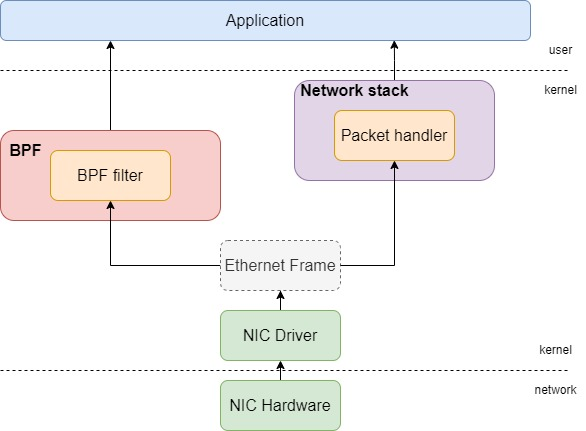
\includegraphics[width=12cm, keepaspectratio=true]{classic_bpf.jpg}
	\caption{Sketch of the functionality of classic BPF}
\end{figure}





\chapter{Methods??}
%M-> Following the particular TFG we discussed and also others, it looks like the main chapter(s) varies name depending on the TFG topic. Also is there a prefered way to distribute this?


\chapter{Results}


\chapter{Conclusion and future work}




%----------
%	BIBLIOGRAPHY
%----------	

%\nocite{*} % Si quieres que aparezcan en la bibliografía todos los documentos que la componen (también los que no estén citados en el texto) descomenta está lína

\clearpage
\addcontentsline{toc}{chapter}{Bibliography}

\printbibliography



%----------
%	ANEX
%----------	

%M-> Mentioned putting some demos and PoCs here...
%

\chapter* {Appendix A}
\pagenumbering{gobble} % Las páginas de los anexos no se numeran

\chapter* {Appendix B}


\end{document}